\usepackage{ucll-code}

\usetikzlibrary{shadows,shapes.multipart}

\title{Default Parameter Values}
\author{Fr\'ed\'eric Vogels}


\lstset{language=c++14}


\begin{document}

\begin{frame}
  \titlepage
\end{frame}

\begin{frame}
  \frametitle{Example Problem}
  \code[font=\small,width=.9\linewidth]{open-file.cpp}
  \begin{center}
    \begin{tabular}{lcc}
      \textbf{Parameter} & \textbf{Optional} & \textbf{Default value} \\
      \toprule
      \tt filename & no & \\
      \tt writable & yes & \tt true \\
      \tt createIfMissing & yes & \tt true \\
    \end{tabular}
  \end{center}
  \begin{itemize}
    \item We don't want the programmer to have to explicitly specify all parameter values
    \item E.g.\ if he wants to create a new writeable file, he should only have to mention the filename
  \end{itemize}
\end{frame}

\begin{frame}
  \frametitle{Typical Solution: Overloading}
  \code[font=\small,width=.9\linewidth]{overloading.cpp}
\end{frame}

\begin{frame}
  \frametitle{Overloading: Problems}
  \code[font=\small,width=.9\linewidth]{overloading-clash.cpp}
  \begin{itemize}
    \item Overloads are not allowed to have same signatures
    \item Overloads above not permitted
  \end{itemize}
\end{frame}

\begin{frame}
  \frametitle{Overloading: Problems}
  \code[font=\small,width=.9\linewidth]{overloading-order.cpp}
  \begin{itemize}
    \item Order of parameters often arbitrary
    \item Unclear from call syntax which parameter gets which value
    \item Need IDE help/documentation to make sense of arguments
    \item Code should be self-documenting
  \end{itemize}
\end{frame}

\begin{frame}
  \frametitle{Overloading: Problems}
  \begin{center}
    \begin{tikzpicture}
      \path[use as bounding box,clip] (-1,-1) rectangle (5,5);
      \draw[-latex] (0,0) -- (5,0) node[at end,anchor=north east,font=\tiny] {number of optional parameters};
      \draw[-latex] (0,0) -- (0,5) node[at end,anchor=south east,font=\tiny,rotate=90] {number of overloads};
      \draw plot[domain=0:4,samples=50,smooth] (\x,1.5^\x-0.8);
    \end{tikzpicture}
  \end{center}
  \vskip-5mm
  \begin{itemize}
    \item Exponential number of overloads required
    \item Lots of boilerplate code
  \end{itemize}
\end{frame}

\begin{frame}
  \frametitle{Default Parameter Values}
  \code[font=\small,width=.9\linewidth]{default-parameter-values.cpp}
  \begin{itemize}
    \item Missing parameters are filled in for you using default values
  \end{itemize}
\end{frame}

\begin{frame}
  \frametitle{Limitations}
  \code[font=\small,width=.9\linewidth]{default-parameter-values-shortcomings.cpp}
  \begin{itemize}
    \item Cannot ``skip'' parameters
    \item If I want to specify 3rd parameter but use the default for the 2nd parameter, I need
          to specify them all anyway
  \end{itemize}
\end{frame}

\begin{frame}
  \frametitle{Caution Advised}
  \code[font=\small,width=.9\linewidth]{default-parameter-values-shortcomings2.cpp}
  \begin{itemize}
    \item No smart type matching
    \item Parameters can never be skipped in \cpp
  \end{itemize}
\end{frame}

\begin{frame}
  \frametitle{Rules: Declaring Functions with Default Parameters}
  \begin{itemize}
    \item If $i$-th parameter has default value, all subsequent parameter must also
          have default values
  \end{itemize}
  \code[font=\small,width=.9\linewidth]{rules-declaring.cpp}
\end{frame}

\begin{frame}
  \frametitle{Rules: Calling Functions with Default Parameters}
  \begin{itemize}
    \item $i$-th argument gets assigned to $i$-th parameter
    \item No intelligence whatsoever
  \end{itemize}
  \vskip5mm
  \code[font=\small,width=.9\linewidth]{rules.cpp}
  \begin{center}
    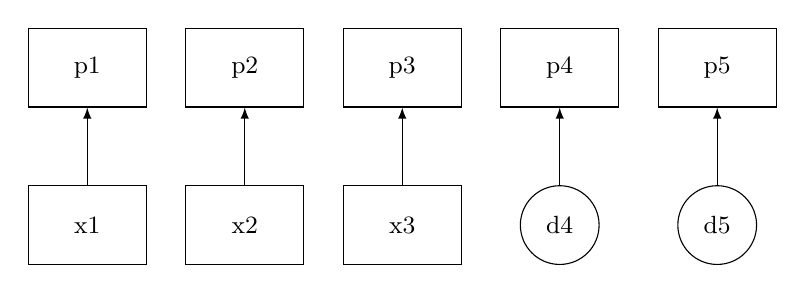
\begin{tikzpicture}[param/.style={draw,minimum width=1.5cm,minimum height=1cm,font=\small},
                        def/.style={draw,circle,minimum size=1cm,font=\small}]
      \foreach[count=\i] \x in {0,2,...,8} {
        \node[param] (param \i) at (\x,0) {p\i};
      }

      \foreach[count=\i] \x in {0,2,...,4} {
        \node[param] (arg \i) at (\x,-2) {x\i};
      }

      \foreach[count=\i] \x in {0,2,...,4} {
        \tikzmath{
          int \j;
          \j = \i + 1;
        }
        \only<\j->{
          \draw[-latex] (arg \i) -- (param \i);
        }
      }

      \foreach[count=\i from 4] \x in {6,8} {
        \tikzmath{
          int \j;
          \j = \i + 1;
        }
        \only<\j->{
          \node[def] (default \i) at (\x,-2) {d\i};
          \draw[-latex] (default \i) -- (param \i);
        }
      }
    \end{tikzpicture}
  \end{center}
\end{frame}

\begin{frame}
  \frametitle{Rules: Single Declaration}
  \begin{itemize}
    \item Default values allowed in both declarations and definition
    \item Compiler may only encounter default values once!
    \item Compiler has to know defaults when you use them
    \item Best practice: put default parameter values in header file
  \end{itemize}
  \vskip5mm
  \begin{overprint}
    \onslide<handout:1|1>
    \code[font=\small,width=.95\linewidth]{single-declaration-1.cpp}
    \onslide<handout:2|2>
    \code[font=\small,width=.95\linewidth]{single-declaration-2.cpp}
    \onslide<handout:3|3>
    \code[font=\small,width=.95\linewidth]{single-declaration-3.cpp}
    \onslide<handout:4|4>
    \code[font=\small,width=.95\linewidth]{single-declaration-4.cpp}
  \end{overprint}
\end{frame}


\end{document}


%%% Local Variables:
%%% mode: latex
%%% TeX-master: "default-parameter-values"
%%% End:
